\documentclass[10pt,conference,compsocconf]{IEEEtran}

\usepackage{hyperref}
\usepackage{graphicx}	% For figure environment


\begin{document}
\title{Writing Scientific Papers and Software}

\author{
  Cheng Soon Ong\\
  \textit{Department of Computer Science, ETH Zurich, Switzerland}
}

\maketitle

\begin{abstract}
  A critical part of scientific discovery is the
  communication of research findings to peers or the general public.
  Mastery of the process of scientific communication improves the
  visibility and impact of research. While this guide is a necessary
  tool for learning how to write in a manner suitable for publication
  at a scientific venue, it is by no means sufficient, on its own, to
  make its reader an accomplished writer. 
  This guide should be a starting point for further development of 
  writing skills.
\end{abstract}

\section{Introduction}

The aim of writing a paper is to infect the mind of your reader with
the brilliance of your idea~\cite{jones08}. 
The hope is that after reading your
paper, the audience will be convinced to try out your idea. In other
words, it is the medium to transport the idea from your head to your
reader's head. 
In the following
section, we show a common structure of scientific papers and briefly
outline some tips for writing good papers in
Section~\ref{sec:tips-writing}.

At that
point, it is important that the reader is able to reproduce your
work~\cite{schwab00,wavelab,gentleman05}. This is why it is also
important that if the work has a computational component, the software
associated with producing the results are also made available in a
useful form. Several guidelines for making your user's experience with
your software as painless as possible is given in
Section~\ref{sec:tips-software}.

This brief guide is by no means sufficient, on its own, to
make its reader an accomplished writer. The reader is urged to use the
references to further improve his or her writing skills.

\section{The Structure of a Paper}
\label{sec:structure-paper}

Scientific papers usually begin with the description of the problem,
justifying why the problem is interesting. Most importantly, it argues
that the problem is still unsolved, or that the current solutions are
unsatisfactory. This leads to the main gist of the paper, which is
``the idea''. The authors then show evidence, using derivations or
experiments, that the idea works. Since science does not occur in a
vacuum, a proper comparison to the current state of the art is often
part of the results. Following these ideas, papers usually have the
following structure:
\begin{description}
\item[Abstract] \ \\
  Short description of the whole paper, to help the
  reader decide whether to read it.
\item[Introduction] \ \\
  Describe your problem and state your
  contributions.
\item[Models and Methods] \ \\
  Describe your idea and how it was implemented to solve
  the problem. Survey the related work, giving credit where credit is
  due.
\item[Results] \ \\
  Show evidence to support your claims made in the
  introduction.
\item[Discussion] \ \\
  Discuss the strengths and weaknesses of your
  approach, based on the results. Point out the implications of your
  novel idea on the application concerned.
\item[Summary] \ \\
  Summarize your contributions in light of the new
  results.
\end{description}


\section{Tips for Good Writing}
\label{sec:tips-writing}

The ideas for good writing have come
from~\cite{editor10,jones08,anderson04}.

\subsection{Getting Help}
One should try to get a draft read by as many friendly people as
possible. And remember to treat your test readers with respect. If
they are unable to understand something in your paper, then it is
highly likely that your reviewers will not understand it
either. Therefore, do not be defensive about the criticisms you get,
but use it as an opportunity to improve the paper. Before your submit
your friends to the pain of reading your draft, please \emph{use a
  spell checker}.

\subsection{Abstract}
The abstract should really be written last, along with the title of
the paper. The four points that should be covered~\cite{jones08}:
\begin{enumerate}
\item State the problem.
\item Say why it is an interesting problem.
\item Say what your solution achieves.
\item Say what follows from your solution.
\end{enumerate}

\subsection{Figures and Tables}

\begin{figure}[tbp]
  \centering
  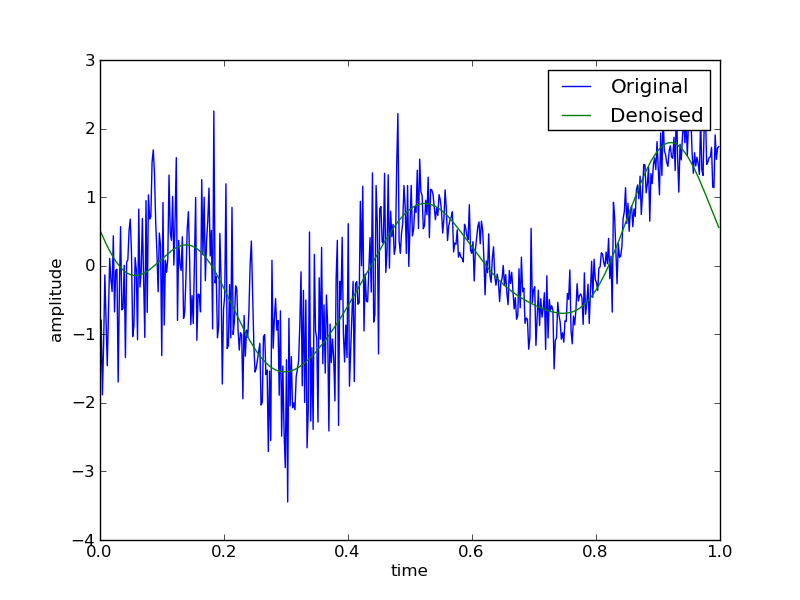
\includegraphics[width=\columnwidth]{denoised_signal_1d}
  \caption{Signal compression and denoising using the Fourier basis.}
  \vspace{-3mm}
  \label{fig:denoise-fourier}
\end{figure}
\begin{figure}[htbp]
  \centering
  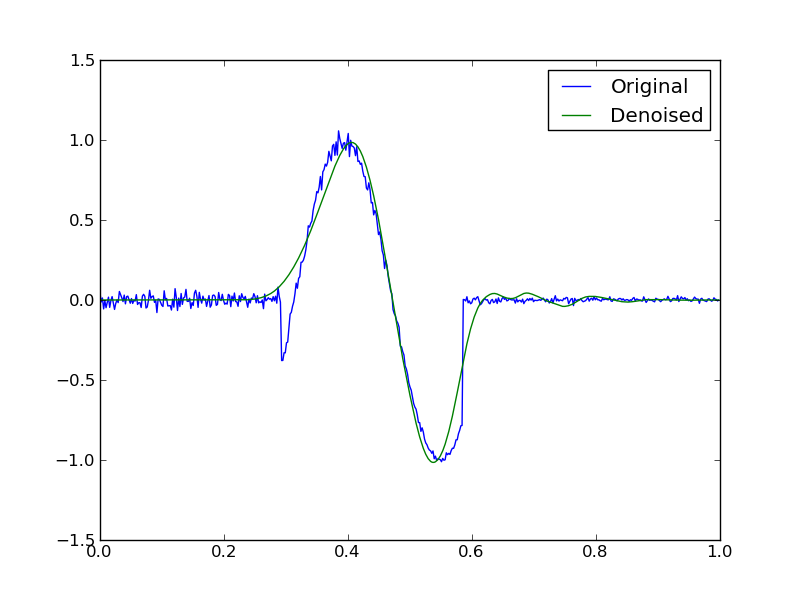
\includegraphics[width=\columnwidth]{local_wdenoised_1d}
  \vspace{-3mm}
  \caption{Signal compression and denoising using the Daubechies wavelet basis.}
  \label{fig:denoise-wavelet}
\end{figure}

Use examples and illustrations to clarify ideas and results. For
example, by comparing Figure~\ref{fig:denoise-fourier} and
Figure~\ref{fig:denoise-wavelet}, we can see the two different
situations where Fourier and wavelet basis perform well. 

\subsection{Models and Methods}
The models and methods
section should describe what was
done to answer the research question, describe how it was done,
justify the experimental design, and
explain how the results were analyzed.

The model refers to the underlying mathematical model or structure which 
you use to describe your problem, or that your solution is based on. 
The methods on the other hand, are the algorithms used to solve the problem. 
In some cases, the suggested method directly solves the problem, without having it 
stated in terms of an underlying model. Generally though it is a better practice to have 
the model figured out and stated clearly, rather than presenting a method without specifying 
the model. In this case, the method can be more easily evaluated in the task of fitting 
the given data to the underlying model.

The methods part of this section, is not a step-by-step, directive,
protocol as you might see in your lab manual, but detailed enough such
that an interested reader can reproduce your
work~\cite{anderson04,wavelab}.

The methods section of a research paper provides the information by
which a study's validity is judged.
Therefore, it requires a clear and precise description of how an
experiment was done, and the rationale
for why specific experimental procedures were chosen.
It is usually helpful to
structure the methods section by~\cite{kallet04methods}:
\begin{enumerate}
\item Layout the model you used to describe the problem or the solution.
\item Describing the algorithms used in the study, briefly including
  details such as hyperparameter values (e.g. thresholds), and
  preprocessing steps (e.g. normalizing the data to have mean value of
  zero).
\item Explaining how the materials were prepared, for example the
  images used and their resolution.
\item Describing the research protocol, for example which examples
  were used for estimating the parameters (training) and which were
  used for computing performance.
\item Explaining how measurements were made and what
  calculations were performed. Do not reproduce the full source code in
  the paper, but explain the key steps.
\end{enumerate}

\subsection{Results}

Organize the results section based on the sequence of table and
figures you include. Prepare the tables and figures as soon as all
the data are analyzed and arrange them in the sequence that best
presents your findings in a logical way. A good strategy is to note,
on a draft of each table or figure, the one or two key results you
want to address in the text portion of the results.
The information from the figures is
summarized in Table~\ref{tab:fourier-wavelet}.

\begin{table*}[htbp]
  \centering
  \begin{tabular}[c]{|l||l|l|l|}
    \hline
    Basis&Support&Suitable signals&Unsuitable signals\\
    \hline
    Fourier&global&sine like&localized\\
    wavelet&local&localized&sine like\\
    \hline
  \end{tabular}
  \caption{Characteristics of Fourier and wavelet basis.}
  \label{tab:fourier-wavelet}
\end{table*}

When reporting computational or measurement results, always
report the mean (average value) along with a measure of variability
(standard deviation(s) or standard error of the mean).


\section{Tips for Good Software}
\label{sec:tips-software}

There is a lot of literature (for example~\cite{hunt99pragmatic} and
\cite{spolsky04software}) on how to write software. It is not the
intention of this section to replace software engineering
courses. However, in the interests of reproducible
research~\cite{schwab00}, there are a few guidelines to make your
reader happy:
\begin{itemize}
\item Have a \texttt{README} file that (at least) describes what your
  software does, and which commands to run to obtain results. Also
  mention anything special that needs to be set up, such as
  toolboxes\footnote{For those who are
  particularly interested, other common structures can be found at
  \url{http://en.wikipedia.org/wiki/README} and
  \url{http://www.gnu.org/software/womb/gnits/}.}.
\item A list of authors and contributors can be included in a file
  called \texttt{AUTHORS}, acknowledging any help that you may have
  obtained. For small projects, this information is often also
  included in the \texttt{README}.
\item Use meaningful filenames, and not \texttt{temp1.py},
  \texttt{temp2.py}. 
\item Document your code. Each file should at least have a short
  description about its reason for existence. Non obvious steps in the
  code should be commented. Functions arguments and return values should be described.
\item Describe how the results presented in your paper can be reproduced.
\end{itemize}


\subsection{\LaTeX{} Primer}
\label{sec:latex-primer}

\LaTeX{} is one of the most commonly used document preparation systems
for scientific journals and conferences. It is based on the idea
that authors should be able to focus on the content of what they are
writing without being distracted by its visual presentation.
The source of this file can be used as a starting point for how to use
the different commands in \LaTeX{}. We are using an IEEE style for
this course.

\subsubsection{Installation}

There are various different packages available for processing \LaTeX{}
documents.
On OSX use Mac\TeX{}
(\url{http://www.tug.org/mactex/}). On Windows, use for example Mik\TeX{} (\url{http://miktex.org/}).

\subsubsection{Compiling \LaTeX{}}
Your directory should contain at least~4 files, in addition to image
files. Images should be in \texttt{.png}, \texttt{.jpg} or
\texttt{.pdf} format.
\begin{itemize}
\item IEEEtran.cls
\item IEEEtran.bst
\item groupXX-submission.tex
\item groupXX-literature.bib
\end{itemize}
Note that you should replace groupXX with your chosen group name.
Then, from the command line, type:
\begin{verbatim}
$ pdflatex groupXX-submission
$ bibtex groupXX-literature
$ pdflatex groupXX-submission
$ pdflatex groupXX-submission
\end{verbatim}
This should give you a PDF document \texttt{groupXX-submission.pdf}.

\subsubsection{Equations}

There are three types of equations available: inline equations, for
example $y=mx + c$, which appear in the text, unnumbered equations
$$y=mx + c,$$
which are presented on a line on its own, and numbered equations
\begin{equation}
  \label{eq:linear}
  y = mx + c
\end{equation}
which you can refer to at a later point (Equation~(\ref{eq:linear})).

\subsubsection{Tables and Figures}

Tables and figures are ``floating'' objects, which means that the text
can flow around it.
Note
that \texttt{figure*} and \texttt{table*} cause the corresponding
figure or table to span both columns.



\section{Summary}

The aim of a scientific paper is to convey the idea or discovery of
the researcher to the minds of the readers. The associated software
package provides the relevant details, which are often only briefly
explained in the paper, such that the research can be reproduced.
To write good papers, identify your key idea, make your contributions
explicit, and use examples and illustrations to describe the problems
and solutions.

\section*{Acknowledgements}
The author thanks Christian Sigg for his careful reading and helpful
suggestions.

\bibliographystyle{IEEEtran}
\bibliography{literature}

\end{document}
